%\documentclass[lecturenotes]{../industrial-development}
\documentclass{../industrial-development}

    \graphicspath{{8-9-project-managment/}}
    \usepackage{multirow}
    \newcommand{\sz}{\footnotesize}
    \newcommand{\zz}{\phantom{0}}
    
    \title{Управление программными проектами}
    \author{Никитин Евгений Сергеевич,\\Быков Михаил Дмитриевич,\\ИВТ-21 МО}
    \date{}
    
    \begin{document}
    
    \begin{frame}
      \titlepage
    \end{frame}

    \section{Программные проекты}

    \subsection{Основные понятия}

    \begin{frame} \frametitle{Продукт}
        \begin{definition}
            \alert{Продукт} "--- основной \alert{конечный результат} проекта (актив), который поставляется заказчику, обычно определен в проектном задании (спецификации) на продукт
        \end{definition}
        \medskip
    \end{frame}
    \lecturenotes

Продукт проекта – материально измеримый результат проекта. Результат встреч с заинтересованными сторонами "--- фиксация продуктов проекта. Описанный продукт проекта определяет результат, которые ожидает увидеть заинтересованные стороны в подтверждение факта завершения реализации проекта.

    \begin{frame} \frametitle{Проект}
        \begin{definition}
            \alert{Проект} "--- временное предприятие, предназначенное для~создания уникальных продуктов, услуг или результатов
        \end{definition}
        \medskip
        В проекте должны быть определены:
        \begin{itemize}
            \item Цели и результаты (область охвата)
            \item Уровень качества
            \item Этапы и сроки выполнения работ
            \item Бюджет
        \end{itemize}
    \end{frame}
    \lecturenotes

Проект "--- временное предприятие,  комплекс взаимно согласованных задач и работ, которые выполняются в течение заданного времени, с использованием ограниченных ресурсов для достижения запланированной цели и получения инновационного продукта определенного качества.

<<Временное>> означает, что у любого проекта есть начало и непременно наступает завершение, когда достигаются поставленные цели, либо возникает понимание, что эти цели не могут быть достигнуты. <<Уникальных>> означает, что создаваемые продукты или услуги существенно отличаются от других аналогичных продуктов и услуг.

Уникальность продуктов или услуг проекта обусловливает необходимость последовательного уточнения их характеристик по мере выполнения проекта.

  \subsection{Управление проектами}

    \begin{frame} \frametitle{Управление проектами}
        \begin{definition}
            \alert{Управление проектами} "--- область деятельности, в ходе которой определяются и достигаются \alert{четкие цели} проекта при балансировании между объёмом работ, ресурсами, временем, качеством и рисками
        \end{definition}
    \end{frame}
    \lecturenotes

Программирование - это творческий процесс. И во все времена задача управления творчеством была актуальна. Инвесторам, менеджерам, государству хотелось бы иметь предсказуемость на счёт того, когда будет выпущен разрабатываемый творческий продукт (будь это книга, самолёт, компьютерная программа или фильм).

Творческая работа может вестись как индивидуально, так и коллективно. При этом в коллективе чаще всего присутствуют специалисты из разных областей (например художник, дизайнер и программист). Управление проектом подразумевает планирование, координацию и контроль работ по проекту для достижения его целей в рамках заданных сроков и бюджета.

Управление проектами дает ощутимые результаты во всех областях приложений, чем и объясняется растущая популярность этой технологии. Для руководителей информационных служб она представляет интерес и как технология, которую полезно внедрить на своих предприятиях, и как средство управления собственными проектами, к которым можно отнести и разработку программного обеспечения, и внедрение тех или иных информационных систем, и прочие изменения, носящие уникальный характер и временные по своей природе.

Проектный подход, безусловно, необходим, как уже было упомянуто, при разработке и выведении на рынок нового продукта, в принципе при реализации какой-либо инновационной идеи. Новый товар или услуга, новый промышленный или социальный инфраструктурный объект, новый сайт или программное обеспечение, разработка региональной программы или подготовка городского праздника – всё это с самого начала потребует применения инструментов проектного менеджмента.
    
Достижение целей проекта может быть реализовано различными способами. Для сравнения этих способов необходимы критерии успешности достижения поставленных целей. Обычно в число основных критериев оценки различных вариантов исполнения проекта входят сроки и стоимость достижения результатов. При этом запланированные цели и качество обычно служат основными ограничениями при рассмотрении и оценке различных вариантов. Конечно, возможно использование и других критериев и ограничений, в частности ресурсных.

    \subsection{Треугольник проекта}

    \begin{frame} \frametitle{Треугольник проекта}
         \centerline{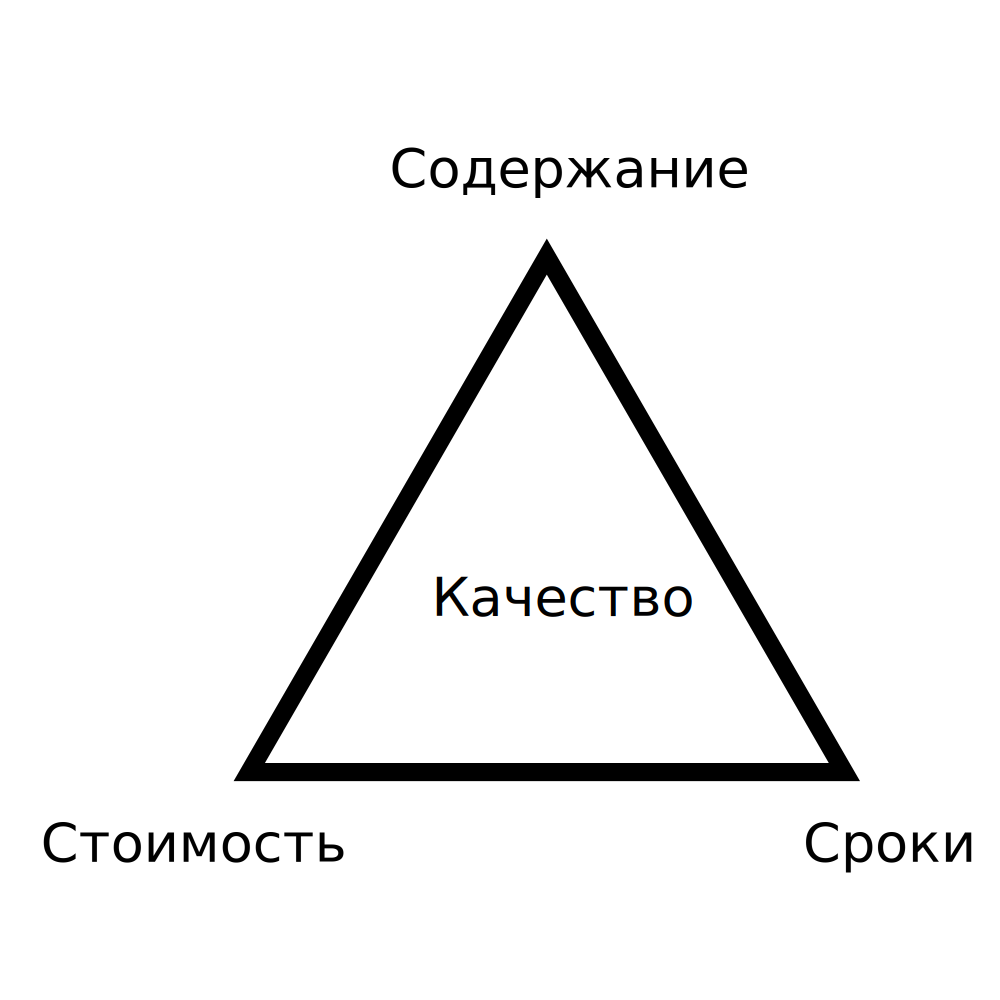
\includegraphics[width=0.8\textwidth]{triangle.pdf}}
    \end{frame}
    \lecturenotes

Бюджет, возможности и график образовывают так называемый железный треугольник управления проектом. Между ними важно научиться балансировать. Ведь, наверное, каждому известны примеры, когда для завершения работы необходим дополнительный бюджет или горят все сроки. Как быть в таких случаях, от чего отказаться и чем пожертвовать?
    
    \begin{frame} \frametitle{Треугольник проекта: идеальный проект}
        \begin{block}{Идеальный проект}
            \begin{itemize}
                \item Соблюдены сроки выполнения
                \item Результат соответствует целям
                \item Затраты в пределах бюджета
            \end{itemize}
        \end{block}
        \medskip
        Не стоит забывать про \alert{качество}!
    \end{frame}
    \lecturenotes

Для управления проектами необходимы рычаги. Влиять на пути достижения результатов проекта, цели, качество, сроки и стоимость исполнения работ можно, выбирая применяемые технологии, состав, характеристики и назначения ресурсов на выполнение тех или иных работ. Таким образом, применяемые технологии и ресурсы проекта можно отнести к основным рычагам управления проектами. Кроме этих основных существуют и вспомогательные средства, предназначенные для управления основными. К таким вспомогательным рычагам управления можно отнести, например, контракты, которые позволяют привлечь нужные ресурсы в нужные сроки. Кроме того, для управления ресурсами необходимо обеспечить эффективную организацию работ. Это касается структуры управления проектом, организации информационного взаимодействия участников проекта, управления персоналом.

    \begin{frame} \frametitle{Треугольник проекта: изменения}
	Если меняется один из его элементов, то это приводит к изменению двух остальных!

	Возможны следующие действия:
	\begin{itemize}
		\item Продлить время работы над проектом
		\item Сократить длительность отдельных этапов
		\item Изменить возможности
	\end{itemize}
    \end{frame}
    \lecturenotes

Треугольником он называется потому что если вы меняете один из его элементов, то это приводит к изменению двух остальных. И то, насколько эффективно вы справитесь с требованиями повлияет на качество в позитивную или негативную сторону.

Предположим, вы разрабатываете проект новой автономной IT-системы. На этапе создания и проектирования вы понимаете, что треугольник трещит по швам, а это не позволит довести проект до завершения. Вы можете предпринять следующие действия:

Продлить время работы над проектом. Вы понимаете, что не сможете создать качественный продукт, поэтому решаете выделить дополнительное время. Это приведет к дополнительным затратам на рабочую силу, однако так как качество "--- ваша главная цель, вы идете на это.

Сократить длительность отдельных этапов. Такой подход может повысить риск неудачи или повлиять на качество продукта. Тем не менее, если к делу подойти творчески и выйти за рамки привычного мышления, можно обнаружить, что некоторые этапы можно объединить или и вовсе убрать без ущерба для проекта.

Изменить возможности. Вы можете убрать из своего проекта некоторые функции, интерфейс и прочие возможности, которые посчитаете менее важными. Это позволит сэкономить бюджет и снизить время работы.


    \begin{frame} \frametitle{Треугольник проекта: на практике}
         \centerline{\includegraphics[width=1\textwidth]{start.jpg}}
    \end{frame}
    \lecturenotes

При работе с любым проектом будут возникать проблемы и придется чем-то жертвовать

В области деятельности под названием <<управление проектами>> существует правило-поговорка о том, что при рассмотрении трех факторов "--- быстро, дешево и хорошо "--- вы можете выбрать только два:

    \begin{frame} \frametitle{Треугольник проекта: крайности}
	\begin{itemize}
		\item Если продукт создается дешевым и при этом быстро, то качество будет хуже
		\item Если продукт дешевый и качественный, значит потребуется значительно больше времени на его создание
		\item Если продукт создается быстро и при этом он качественный, придется повышать его цену
	\end{itemize}
    \end{frame}
    \lecturenotes

Если вы создаете продукт дешевым и при этом быстро, то жертвуете качеством.

Если продукт дешевый и качественный, значит потребуется значительно больше времени на его создание.

Если продукт создается быстро и при этом он качественный, придется повышать его цену.
    
    \section{Жизненный цикл проекта}

    \subsection{Инициация}

    \begin{frame} \frametitle{Жизненный цикл проекта}
	\begin{definition}
		\alert{Жизненный цикл проекта} "--- это стадии процесса, охватывающие различные состояния системы, начиная с момента возникновения необходимости в такой системе и заканчивая её полным выводом из эксплуатации
	\end{definition}
    \end{frame}
    \lecturenotes
	-

    \begin{frame} \frametitle{Схема жизненного цикла}
         \centerline{\includegraphics[width=0.7\textwidth]{manageproject.pdf}}
    \end{frame}
    \lecturenotes

	На фазе инициации проекта необходимо понять, что и зачем мы будем делать "--- разработать концепцию проекта. Фаза планирования определяет, как мы будем это делать. На фазе исполнения происходит материализация наших идей в виде документированного и протестированного программного продукта. И, наконец, на фазе завершения мы должны подтвердить, что мы разработали именно тот продукт, который задумали в концепции проекта, а также провести приемо-сдаточные испытания (ПСИ) продукта на предмет соответствия его свойств, определенным ранее требованиям.
Как правило, редкий проект выполняется в соответствие с первоначальными планами, поэтому важным элементом фазы завершения является <<обратная связь>>: анализ причин расхождения и усвоение уроков на будущее. Помним, что управляющая система без обратной связи не может быть устойчивой.

    \begin{frame} \frametitle{Инициация проекта}
	\begin{definition}
		\alert{Инициация проекта} "--- стадия процесса управления проектом, результатом которой является санкционирование начала проекта или очередной фазы его жизненного цикла
	\end{definition}
	Процессы инициации:

	\begin{itemize}
		\item Уточняются первоначальное описание содержания
		\item Определяются ресурсы, которые организация планирует вложить в проект
		\item Выбирается менеджер проекта, если он еще не назначен
		\item Документируются исходные допущения и ограничения
	\end{itemize}
    \end{frame}
    \lecturenotes

	состоит из процессов, способствующих формальной авторизации начала нового проекта или фазы проекта. Процессы инициации часто выполняются вне рамок проекта и связаны с организационными, программными или портфельными процессами. В ходе процесса инициации уточняются первоначальное описание содержания и ресурсы, которые организация планирует вложить. На этом этапе также выбирается менеджер проекта, если он еще не назначен, и документируются исходные допущения и ограничения. Эта информация заносится в Устав проекта и, если он одобряется, проект официально авторизуется.

    \begin{frame} \frametitle{Устав проекта}
	\begin{definition}
		\alert{Устав проекта (концепция)} "--- документ, выпущенный инициатором или спонсором проекта, который формально узаконивает существование проекта и предоставляет менеджеру проекта полномочия использовать организационные ресурсы в операциях проекта
	\end{definition}
    \end{frame}
    \lecturenotes
-

    \begin{frame} \frametitle{Приоритет проекта}
	Приоритет проекта определяться на основе оценки трех его характеристик:
	
	\begin{itemize}
		\item Финансовая ценность
		\item Стратегическая ценность
		\item Уровень рисков
	\end{itemize}
    \end{frame}
    \lecturenotes
    В компании, которая принимает решение о старте того или иного проекта разработки ПО, должна существовать единая система критериев для оценки его значимости. Система критериев должна позволять из множества возможных для реализации проектов выбрать наиболее приоритетные для компании.

    \begin{frame} \frametitle{Финансовая ценность}
	\begin{itemize}
		\item Высокая. Ожидаемая окупаемость до 1 года
		\item Выше среднего. Ожидаемая окупаемость проекта от 1 года до 3 лет
		\item Средняя. Проект позволяет улучшить эффективность производства в Компании и потенциально может снизить расходы компании не менее чем на 30\,\%
		\item Низкая. Проект немного снижает расходы компании не менее чем на 10\,\%
	\end{itemize}
    \end{frame}
    \lecturenotes

Высокая. Ожидаемая окупаемость до 1 года. Ожидаемые доходы от проекта не менее чем в 1.5 раз превышают расходы. Все допущения при проведении этих оценок четко обоснованны.

Выше среднего. Ожидаемая окупаемость проекта от 1 года до 3 лет. Ожидаемые доходы от проекта не менее чем в 1.3 раза превышают расходы. Большинство допущений при проведении этих оценок имеют под собой определенные основания.

Средняя. Проект позволяет улучшить эффективность производства в Компании и потенциально может снизить расходы компании не менее чем на 30\,\%. Проект может иметь информационную ценность или помочь лучше контролировать бизнес.

Низкая. Проект немного снижает расходы компании не менее чем на 10\,\% и дает некоторые улучшения производительности производства.

    \begin{frame} \frametitle{Стратегическая ценность}
	\begin{itemize}
		\item Высокая. Обеспечивает стратегическое преимущество
		\item Выше среднего. Создает временные конкурентные преимущества
		\item Средняя. Поддерживается доверие рынка к компании
		\item Низкая. Стратегическое воздействие отсутствует или незначительно
	\end{itemize}
    \end{frame}
    \lecturenotes

Высокая. Обеспечивает стратегическое преимущество, дает устойчивое увеличение рынка или позволяет выйти на новый рынок. Решает значительные проблемы, общие для большинства важных клиентов. Повторение конкурентами затруднено или потребует от 1 до 2 лет.

Выше среднего. Создает временные конкурентные преимущества. Выполнение обязательств перед многими важными клиентами. Конкурентное преимущество может быть удержано в течение 1 года.

Средняя. Поддерживается доверие рынка к компании. Повышает мнение клиентов о качестве предоставляемых услуг или способствует выполнению обязательств перед несколькими клиентами. Конкуренты уже имеют или способны повторить новые возможности в пределах года.

Низкая. Стратегическое воздействие отсутствует или незначительно. Влияние на клиентов несущественно. Конкуренты могут легко повторить результаты проекта.

    \begin{frame} \frametitle{Концепция проекта}
	Концепция проекта содержит следующие разделы:
	\begin{itemize}
		\item Название проекта
		\item Цели проекта
		\item Результаты проекта
		\item Допущения и ограничения
		\item Ключевые участники и заинтересованные стороны
		\item Ресурсы проекта
		\item Сроки
		\item Риски
		\item Критерии приемки
		\item Обоснование полезности проекта
	\end{itemize}
    \end{frame}
    \lecturenotes

У каждого проекта должна быть концепция. Если проект небольшой, то для изложения концепции часто достаточно несколько абзацев. Однако, стартовать проект без концепции, это все равно, что отправлять корабль в плавание, не определив для него пункт назначения.

Концепция проекта разрабатывается на основе анализа потребностей бизнеса. Главная функция документа "--- подтверждение и согласование единого видения целей, задач и результатов всеми участниками проекта. Концепция определяет что и зачем делается в проекте.

Концепция проекта это ключевой документ, который используется для принятия решений в ходе всего проекта, а также на фазе приемки — для подтверждения результата. Она содержит, как правило, следующие разделы:

Название проекта
Цели проекта
Результаты проекта
Допущения и ограничения
Ключевые участники и заинтересованные стороны
Ресурсы проекта
Сроки
Риски
Критерии приемки
Обоснование полезности проекта

    \begin{frame} \frametitle{Цели проекта}
    Цели проекта должны отвечать на вопрос, зачем данный проект нужен
    
	Целями проекта могут быть:
	\begin{itemize}
		\item Изменения в компании
		\item Реализация стратегических планов
		\item Выполнение контрактов
		\item Разрешение специфических проблем
	\end{itemize}
    \end{frame}
    \lecturenotes

Цели проекта должны отвечать на вопрос, зачем данный проект нужен. Цели проекта должны описывать бизнес-потребности и задачи, которые решаются в результате исполнения проекта. Целями проекта могут быть:

Изменения в Компании. Например, автоматизация ряда бизнес-процессов для повышения эффективности основной производственной деятельности
Реализация стратегических планов. Например, завоевание значительной доли растущего рынка за счет вывода на него нового продукта.

Выполнение контрактов. Например, разработка программного обеспечения по заказу.

Разрешение специфических проблем. Например, доработка программного продукта в целях приведения его в соответствие с изменениями в законодательстве.

Цели должны быть значимыми (направленными на достижение стратегических целей Компании), конкретными (специфичными для данного проекта), измеримыми (т.е иметь проверяемые количественные оценки), реальными (достижимыми). Четкое определение бизнес-целей важно, поскольку существенно влияет на все процессы и решения в проекте. Проект должен быть закрыт, если признается, что достижение цели невозможно или стало нецелесообразным. Например, если реальные затраты на проект будут превосходить будущие доходы от его реализации.

    \begin{frame} \frametitle{Результаты проекта}
	\begin{itemize}
		\item Что получит заказчик в результате проекта
		\item Что конкретно будет произведено по окончании проекта
		\item Краткое описание и при необходимости ключевые свойства и/или характеристики продукта/услуги
	\end{itemize}
    \end{frame}
    \lecturenotes

Результаты проекта отвечают на вопрос, что должно быть получено после его завершения. Результаты проекта должны определять:

Какие именно бизнес-выгоды получит заказчик в результате проекта.

Какой продукт или услуга. Что конкретно будет произведено по окончании проекта.

Высокоуровневые требования. Краткое описание и при необходимости ключевые свойства и/или характеристики продукта/услуги.

Следует помнить, что результаты проекта должны быть измеримыми. Это означает, что при оценке результатов проекта должна иметься возможность сделать заключение достигнуты оговоренные в концепции результаты или нет.

    \begin{frame} \frametitle{Допущения и ограничения}
	\begin{itemize}
		\item Специфические нормативные требования
		\item Специфические технические требования
		\item Специфические требования к защите информации
		\item Требования к системе, которые могут ожидаться заказчиком по умолчанию, но не включаются в рамки данного проекта
	\end{itemize}
    \end{frame}
    \lecturenotes

Данный раздел описывает исходные допущения и ограничения. Допущения, как правило, тесно связаны с управлением рисками, о котором мы будем говорить далее. В разработке ПО часто приходится формулировать риски в виде допущений, тем самым передавая его заказчику. Например, оценивая проект разработки и внедрения по схеме с фиксированной ценой, мы должны записать в допущения предположение о том, что стоимость лицензий на стороннее ПО не изменится, до завершения проекта.

Ограничения, как правило, сокращают возможности проектной команды в выборе решений. В частности они могут содержать:

Специфические нормативные требования. Например, обязательная сертификация продукта, услуги на соответствие определенным стандартам.

Специфические технические требования. Например, разработка под заданную программно-аппаратную платформу.

Специфические требования к защите информации.

В этом разделе также уместно сформулировать те требования к системе, которые могут ожидаться заказчиком по умолчанию, но не включаются в рамки данного проекта. Например, в данный раздел может быть включен пункт о том, что разработка программного интерфейса (API) для будущей интеграции с другими системами заказчика не входит в задачи данного проекта.

    \begin{frame} \frametitle{Ключевые участники}
	\begin{itemize}
		\item Спонсор проекта 
		\item Заказчик проекта
		\item Пользователи результатов проекта
		\item Куратор проекта
		\item Руководитель проекта
		\item Соисполнители проекта
		\item Субподрядчики и поставщики
	\end{itemize}
    \end{frame}
    \lecturenotes

Одна из задач фазы инициации проекта это выявить и описать всех его участников. Согласно к участникам проекта относятся все заинтересованные стороны (stakeholders), лица и организации, например заказчики, спонсоры, исполняющая организация, которые активно участвуют в проекте или чьи интересы могут быть затронуты при исполнении или завершении проекта. Участники также могут влиять на проект и его результаты поставки.

К ключевым участникам программного проекта, как правило, относятся:

Спонсор проекта — лицо или группа лиц, предоставляющая финансовые ресурсы для проекта в любом виде.

Заказчик проекта — лицо или организация, которые будут использовать продукт, услугу или результат проекта. Следует учитывать, что заказчик и спонсор проекта не всегда совпадают.

Пользователи результатов проекта.

Куратор проекта — представитель исполнителя, уполномоченный принимать решение о выделении ресурсов и изменениях в проекте.

Руководитель проекта — представитель исполнителя, ответственный за реализацию проекта в срок, в пределах бюджета и с заданным качеством.

Соисполнители проекта. Субподрядчики и поставщики.

    \begin{frame} \frametitle{Ресурсы}
	\begin{itemize}
		\item Людские ресурсы и требования к квалификации персонала
		\item Оборудование, услуги, расходные материалы, лицензии на ПО, критические компьютерные ресурсы
		\item Бюджет проекта
	\end{itemize}
         \centerline{\includegraphics[width=0.7\textwidth]{ress.png}}
    \end{frame}
    \lecturenotes

Для того чтобы понять, сколько будет стоить реализация программного проекта, требуется определить и оценить ресурсы необходимые для его выполнения:

Людские ресурсы и требования к квалификации персонала.

Оборудование, услуги, расходные материалы, лицензии на ПО, критические компьютерные ресурсы.

Бюджет проекта. План расходов и, при необходимости, предполагаемых доходов проекта с разбивкой по статьям и фазам/этапам проекта.

Специфика программного проекта заключается в том, что людские ресурсы вносят основной вклад в его стоимость. Все остальные затраты, как правило, незначительны, по сравнению с этим расходами. О том, как следует подходить к оценкам трудозатрат на реализацию проекта разработки ПО, мы будем подробно говорить в следующих лекциях. На фазе инициации хорошей считается оценка трудозатрат с точностью от -50\,\% до +100\,\%.

Необходимо помнить, что помимо непосредственно программирования в проекте разработки ПО есть много других процессов, которые требуют ресурсы соответствующей квалификации, а само программирование составляет лишь четверть всех затрат. Распределение трудозатрат по основным производственным процессам при современном процессе разработки ПО выглядит в среднем следующим образом:
 
Поэтому, если по вашей оценки для реализации требуемой функциональности в проекте необходимо написать 10 KSLOC (тысяч строк исходного программного кода), а ваши программисты пишут в среднем по 100 SLOC в день, то общие трудозатраты на проект будут не 100 чел.*дней, а не менее чем 400 чел.*дней. Остальные ресурсы потребуются на анализ и уточнение требований, проектирование, документирование, тестирование и другие проектные работы.

    \begin{frame} \frametitle{Сроки}
         \centerline{\includegraphics[width=0.7\textwidth]{times.png}}
	Формула Боэма: T = 2,5 (N ч.*м.)1/3

T – время первой поставки

N ч.*м - объем работ в человеко-месяцах
    \end{frame}
    \lecturenotes

Ф. Брукс писал: <<Чтобы родить ребенка требуется девять месяцев независимо от того, сколько женщин привлечено к решению данной задачи. Многие задачи программирования относятся к этому типу, поскольку отладка по своей сути носит последовательный характер>>.

Там же Брукс приводит исключительно полезную, но почему-то редко применяемую, эмпирическую формулу оценки срока проекта по его трудоемкости. Формула была выведена Барии Боэмом (Barry Boehm) на основе анализа результатов 63 проектов разработки ПО, в основном в аэрокосмической области. Согласно этой формуле, для проекта, общая трудоемкость которого составляет N ч.*м. (человеко-месяцев), пожно утверждать что:

Существует оптимальное, с точки зрения затрат, время выполнения графика для первой поставки: T = 2,5 (N ч.*м.)1/3. То есть оптимальное время в месяцах пропорционально кубическому корню предполагаемого объема работ в человеко-месяцах. Следствием является кривая, дающая оптимальную численность проектной команды (Рисунок 15).
Кривая стоимости медленно растет, если запланированный график длиннее оптимального. Работа занимает все отведенное для нее время.

Кривая стоимости резко растет, если запланированный график короче оптимального. Практически ни один проект невозможно завершить быстрее, чем за 3/4 расчетного оптимального графика вне зависимости от количества занятых в нем!

Этот примечательный результат дает менеджеру программного проекта солидное подкрепление, когда высшее руководство требует принятия невозможного графика.

    \begin{frame} \frametitle{Контрольная точка}
	\begin{itemize}
		\item Важный момент или событие в расписании проекта, отмечающее достижение заданного результата и/или начало / завершение определенного объема работы
		\item Характеризуется датой и объективными критериями ее достижения
	\end{itemize}
    \end{frame}
    \lecturenotes

Контрольная точка — важный момент или событие в расписании проекта, отмечающее достижение заданного результата и/или начало / завершение определенного объема работы. Каждая контрольная точка характеризуется датой и объективными критериями ее достижения.

Как мы говорили ранее, современный проект разработки ПО должен реализовываться с применением инкрементального процесса. В этом случае контрольные точки должны соответствовать выпуску каждой промежуточной версии ПО, в которой будет реализована и протестирована определенная часть конечной функциональности программного продукта. В зависимости от сложности и масштаба проекта продолжительность одной итерации может составлять от 2 до 8 недель.

    \begin{frame} \frametitle{Критерии приемки}
	Критерии приемки определяют числовые значения характеристик системы, которые должны быть продемонстрированы по результатам приемосдаточных испытаний или опытной эксплуатации и однозначно свидетельствовать о достижении целей проекта.
    \end{frame}
    \lecturenotes

Критерии приемки должны определять числовые значения характеристик системы, которые должны быть продемонстрированы по результатам приемосдаточных испытаний или опытной эксплуатации и однозначно свидетельствовать о достижении целей проекта.

    \begin{frame} \frametitle{Обоснование полезности проекта}
	\begin{itemize}
		\item Для кого предназначены результаты проекта
		\item Описание текущей ситуации <<As Is>>. Какие у потенциального заказчика существуют проблемы
		\item Каким образом результаты проекта решают эти проблемы (<<To Be>>)
		\item Насколько значимо для клиента решение данных проблем (оценка экономического эффекта)
		\item Какие преимущества в итоге из этого может извлечь компания-исполнитель проекта
	\end{itemize}
    \end{frame}
    \lecturenotes

Этот раздел концепции должен содержать краткое технико-экономическое обоснование проекта:

Для кого предназначены результаты проекта.

Описание текущей ситуации <<As Is>>. Какие у потенциального заказчика существуют проблемы.

Каким образом результаты проекта решают эти проблемы (<<To Be>>).

Насколько значимо для клиента решение данных проблем (оценка экономического эффекта).

Какие преимущества в итоге из этого может извлечь компания-исполнитель проекта.

    \begin{frame} \frametitle{Итеративность и инкрементность}
	Итеративность
	\begin{itemize}
		\item Требования к системе и ее архитектура прорабатываются не один раз, а постепенно уточняются от итерации к итерации
		\item На каждой итерации происходит полный цикл процессов разработки: уточнение требований, проектирование, кодирование, тестирование и документирование
	\end{itemize}
	Инкрементность
	\begin{itemize}
		\item Результатом каждой итерации является версия ПО, которая реализует часть функциональности будущего программного продукта
		\item После каждой итерации происходит прирост требуемого функционала, а нереализованных функций будущего продукта остается все меньше
	\end{itemize}
    \end{frame}
    \lecturenotes

В современных моделях разработки ПО реализация осуществляется на основе сочетания итеративного и инкрементного подходов.


Сочетание итеративности и инкрементности обеспечивает эффективность разработки и существенное снижение рисков по ходу проекта. Об этом мы еще будем говорить.
В современных моделях разработки ПО реализация осуществляется на основе сочетания итеративного и инкрементного подходов.
Итеративность предполагает, что требования к системе и ее архитектура прорабатываются не один раз, а постепенно уточняются от итерации к итерации. Это означает, что на каждой итерации происходит полный цикл процессов разработки: уточнение требований, проектирование, кодирование, тестирование и документирование.
Инкрементность состоит в том, что результатом каждой итерации является версия ПО, которая реализует часть функциональности будущего программного продукта и может быть введена в тестовую или опытную эксплуатацию, а также оценена заказчиком и будущими пользователями. Это означает, что после каждой итерации происходит прирост требуемого функционала, а нереализованных функций будущего продукта остается все меньше.





    \subsection{Планирование}

    \begin{frame} \frametitle{Планирование}
        Помимо работ, непосредственно направленных на создание программного обеспечения, в плане проекта должны быть предусмотрены необходимые ресурсы для обеспечения работ по следующим процессам:
	\begin{itemize}
		\item управление содержанием
		\item управление конфигурациями
        \item управление качеством
        \item управление рисками
        \item управление проектом
	\end{itemize}
    \end{frame}
    \lecturenotes
    -

    \begin{frame} \frametitle{Уровни декомпозиции}
        \begin{itemize}
            \item Продукты проекта
            \begin{itemize}
                \item Компоненты, из которых эти продукты состоят
                \begin{itemize}
                    \item Действия, которые компоненты должны реализовывать
                \end{itemize}
            \end{itemize}
        \end{itemize}
    \end{frame}
    \lecturenotes
    
    Это означает, что на верхнем уровне декомпозиции нашего проекта должны находиться продукты проекта, а на следующем уровне — компоненты, из которых эти продукты состоят. Компоненты далее могут быть декомпозированы на <<фичи>> — функции, которые они должны реализовывать.

    \begin{frame} \frametitle{Иерархическая структура работ (ИСР)}
        \begin{definition}
            \alert{Иерархическая структура работ (ИСР)} "--- ориентированная на результат иерархическая декомпозиция работ, выполняемых командой проекта для достижения целей проекта и необходимых результатов
        \end{definition}
    
        ИСР делит проект на подпроекты, пакеты работ, подпакеты
        \end{frame}
        \lecturenotes
    
    <<Если не получается проглотить слона целиком, то его надо порезать на отбивные>>. Человечество пока не придумало ничего более эффективного для решения сложной задачи, чем анализ и ее декомпозиция на боле простые подзадачи, которые, в свою очередь, могут быть разделены на еще боле простые подзадачи и так далее. Получается некоторая иерархическая структура, дерево, в корне которого находится проект, а на листьях элементарные задачи или работы, которые надо выполнить, чтобы завершить проект в условиях заданных ограничений. Согласно:
    
    Иерархическая структура работ (ИСР) (Work /Breakdown Structure, WBS) "--- ориентированная на результат иерархическая декомпозиция работ, выполняемых командой проекта для достижения целей проекта и необходимых результатов. С ее помощью структурируется и определяется все содержание проекта. Каждый следующий уровень иерархии отражает более детальное определение элементов проекта.
    
    ИСР делит проект на подпроекты, пакеты работ, подпакеты. Каждый следующий уровень декомпозиции обеспечивает последовательную детализацию содержания проекта, что позволяет производить оценку сроков и объемов работ. ИСР должна включать все промежуточные и конечные продукты. 

    \begin{frame} \frametitle{Пример ИСР}
        \begin{itemize}
            \item Проект разработки <<Автоматизированной системы продажи документации>>
            \begin{itemize}
                \item Подготовка технического задания на автоматизацию
                \begin{itemize}
                    \item Проведение аналитического обследования
                    \item Разработка функциональных требований

                    ...
                    \item ТЗ утверждено 
                \end{itemize}
                ...
                \item Разработка и тестирование прикладного ПО
                \begin{itemize}
                    \item Установка и конфигурирование рабочей среды
                    \item Проектирование и разработка ПО
                    \item Авторизация и аутентификация пользователей
                    \item Разработка подсистемы заказа документации
                    \item Просмотр каталога продуктов
                    \item Заказ выбранных продуктов
                \end{itemize}
            \end{itemize}
        \end{itemize}
    \end{frame}
    \lecturenotes    
    Выделение компонентов, составляющих программный продукт, это элемент высокоуровневого проектирования, которое мы должны выполнить на фазе планирования проекта, не дожидаясь проработки всех функциональных требований к разрабатываемому ПО. Компонентами могут быть как прикладные подсистемы, так и инфраструктурные, например, подсистема логирования, безопасности, библиотека визуальных компонентов GUI.

    \begin{frame} \frametitle{Функции ИСР}
        \begin{itemize}
            \item Измерение степени достижения результатов проекта
            \item Выявление отклонений от базового плана
            \item Обеспечение представления всех участников проекта относительно того, как будет делаться проект
        \end{itemize}
    \end{frame}
    \lecturenotes
    ИСР является одним из основных инструментов (средств) в механизме управления проектом, с помощью которого измеряется степень достижения результатов проекта. Важнейшая ее функция это обеспечить консистентное представление всех у частников проекта относительно того, как будет делаться проект. В последующем базовый план будет служить ориентиром для сравнения с текущим исполнением проекта и выявления отклонений для целей управления. 

    \begin{frame} \frametitle{Планирование управления содержанием}
        \begin{itemize}
            \item Определить источники запросов на изменение
            \item Установить порядок анализа, оценки и утверждения/отклонения изменения содержания
            \item Определить порядок документирования изменений содержания
            \item Определить порядок информирования об изменении содержания
        \end{itemize}
    \end{frame}
    \lecturenotes
Одна из распространенных <<болезней>> программных проектов называется <<ползучий фичеризм>>. Это, когда к изначально спроектированной будке для любимой собаки сначала пристраивают сарайчик для хранения садового инвентаря, а потом и домик в несколько этажей для ее хозяина. И все это пытаются построить на одном и том же фундаменте и из тех же самых материалов. Эта болезнь стала причиной летального исхода многих проектов разработки ПО.

Поэтому, сразу, как только удалось стабилизировать и согласовать ИСР, необходимо разработать план управления содержанием проекта. Для этого следует:

Определить источники запросов на изменение.

Установить порядок анализа, оценки и утверждения/отклонения изменения содержания.

Определить порядок документирования изменений содержания.

Определить порядок информирования об изменении содержания.

Первая задача, которую необходимо решить при анализе запроса на изменения — выявить объекты изменений: требования, архитектура, структуры данных, исходные коды, сценарии тестирования, пользовательская документация, проч. Затем требуется спроектировать и детально описать изменения во всех выявленных объектах. И наконец, следует оценить затраты на внесение изменений, тестирование изменений и регрессионное тестирование продукта и их влияние на сроки проекта.

Эта работа, которая потребует затрат рабочего времени и порой значительных разных специалистов: аналитиков, проектировщиков, разработчиков, тестировщиков, наконец, менеджера проекта. Поэтому эта работа должна обязательно быть учтена в плане.

    \begin{frame} \frametitle{Планирование организационной структуры}
        \begin{definition}
            \alert{Организационная структура} "--- это согласованное и утвержденное распределение ролей, обязанностей и целей деятельности ключевых участников проекта
        \end{definition}
        Организационная структура включает в себя:
        \begin{itemize}
            \item систему рабочих взаимоотношений между рабочими группами проекта
            \item систему отчетности
            \item оценки хода выполнения проекта
            \item систему принятия решений
        \end{itemize}
    \end{frame}
    \lecturenotes
    Организационная структура это согласованное и утвержденное распределение ролей, обязанностей и целей деятельности ключевых участников проекта. Она в обязательном порядке должна включать в себя систему рабочих взаимоотношений между рабочими группами проекта, систему отчетности, оценки хода выполнения проекта и систему принятия решений. Следует помнить, что организационная структура проекта — <<живой>> организм. Она начинает складываться на стадии планирования и должна меняться по ходу проекта.

    И еще. Нестабильность организационной структуры — частая смена исполнителей — может стать серьезной проблемой в управлении проектом, поскольку, существует цена замены, которая определяется временем вхождения нового участника в контекст проекта.

    \begin{frame} \frametitle{Планирование управления конфигурациями}
        \begin{itemize}
            \item Обеспечение единого хранилища всей проектной документации и разрабатываемого программного кода
            \item Обеспечение сохранности и восстановление проектной информации после сбоя
            \item Настройка рабочих станций и серверов, используемых участниками проектной команды
            \item Организация сборки промежуточных выпусков системы, а также ее конечного варианта
        \end{itemize}
    \end{frame}
    \lecturenotes
Конфигурационное управление один из важных процессов производства программного обеспечения. Об этой области знаний написана не одна книга. Мы будем говорить только о том, что эта работа должна быть спланирована.

План проекта должен включать в себя работы по обеспечению единого хранилища всей проектной документации и разрабатываемого программного кода, обеспечению сохранности и восстановление проектной информации после сбоя. Работы по настройке рабочих станций и серверов, используемых участниками проектной команды, тоже должны войти в план. Кроме этого в плане должны содержаться работы, необходимые для организации сборки промежуточных выпусков системы, а также ее конечного варианта.

Эти работы, как правило, выполняет один человек — инженер по конфигурациям. Если проект небольшой, то эта роль может быть дополнительной для одного из программистов. Я как-то видел, что эту роль выполнял менеджер проекта. <<Размазывать>> эту работу на всех участников проекта, во-первых, неэффективно. Установка и конфигурирование среды разработки, например, баз данных и серверов приложений, требует определенных компетенций и знаний особенностей конкретных версий продуктов. Если эти навыки придется осваивать всем разработчикам, то на это уйдет слишком много рабочего времени. Во-вторых, <<размазывание>> работ по управлению конфигурациями может привести к коллективной безответственности, когда никто не знает, от чего не собирается проект и как откатиться к консистентной версии.

Управление конфигурациями может многократно усложниться, если проектной команде параллельно с разработкой новой функциональности продукта приходится поддерживать несколько релизов этого продукта, которые были установлены ранее у разных клиентов. Все эти работы должны быть учтены в плане проекта.

    \begin{frame} \frametitle{Планирование управления качеством}
        \begin{itemize}
            \item Объективная проверка соответствия продукта применяемым стандартам
            \item Определение отклонений по качеству
            \item План управления рисками
            \item Оценку трудоемкости и сроков работ
        \end{itemize}
    \end{frame}
    \lecturenotes
Обеспечение качества еще одна из базовых областей знаний в программной инженерии. Относительно того, что такое качество ПО и как его эффективно обеспечивать, можно рассуждать очень и очень долго. В нашем курсе мы ограничимся утверждением о том, что обеспечение качества это важная работа, которая должна быть спланирована заранее и выполняться по ходу всего программного проекта, а не только во время приемо-сдаточных испытаний.

При планировании этой работы необходимо понимать, что продукт проекта не должен обладать наивысшим возможным качеством, которое недостижимо за конечное время. Необходимое качество продукта определяется требованиями к нему. И еще. Основная задача обеспечения качества это не поиск ошибок в готовом продукте (выходной контроль) а их предупреждение в процессе производства. Для примера, гладкость обработки детали на токарном станке только случайно может оказаться соответствующей требуемому качеству в 1 микрон, если шпиндель, в котором крепится деталь, плохо центрован.

План управления качеством должен включать в себя следующие работы:

Объективную проверку соответствия программных продуктов и технологических операций применяемым стандартам, процедурам и требованиям.

Определение отклонений по качеству, выявление их причин, применение мер по их устранению, а также контроль исполнения принятых мер и их эффективности.

Представление высшему руководству независимой информации о несоответствиях, не устраняемых на уровне проекта.

Помимо перечисленных разделов план проекта должен включать еще:

План управления рисками

Оценку трудоемкости и сроков работ


    \begin{frame} \frametitle{Базовое расписание проекта}
        \begin{definition}
            \alert{Базовое расписание} "--- утвержденный план-график с указанными временными фазами проекта, контрольными точками и элементами иерархической структуры работ
        \end{definition}
    \end{frame}
    \lecturenotes
После определения трудоемкости работ необходимо определить график их выполнения и общие сроки реализации проекта — составить расписание работ по проекту. Базовое расписание — утвержденный план-график с указанными временными фазами проекта, контрольными точками и элементами иерархической структуры работ.

Базовое расписание может быть наиболее наглядно представлено диаграммой Ганта. В этой диаграмме плановые операции или элементы иерархической структуры работ перечислены с левой стороны, даты отображаются сверху, а длительность операций показана горизонтальными полосками от даты начала до даты завершения.

Базовое расписание это, как правило, элемент контракта с заказчиком. Контрольные точки (вехи) должны служить точками анализа состояния проекта и принятия решения <<GO/NOT GO>>, поэтому они должны зримо демонстрировать статус проекта. Контрольная точка <<Проектирование завершено>> — плохо. Наиболее эффективный подход — метод последовательных поставок: контрольная точка <<Завершено тестирование требований 1, 3, 5, 7>>

Если работы не связаны между собой, то любую из них мы можем начинать и завершать, когда нам удобно. Все работы можно делать параллельно и в этом случае минимальная длительность проекта равна длительности самой долгой работы. Однако, на практике между работами существуют зависимости, которые могут быть <<жесткими>>, например, анализ — проектирование — кодирование — тестирование и документирование конкретной функции; или <<нежесткими>>, которые могут пересматриваться или смягчаться. Например, последовательное выполнение задач конкретным исполнителем (можно перепланировать на другого исполнителя) или разработка базового ПО, которая должна предшествовать разработке прикладного ПО. В этом случае можно создавать <<заглушки>> эмулирующие работу базового ПО. Таким образом, диаграмма Ганта для расписания проекта выглядит как гамак, составленный из множества цепочек взаимосвязанных работ с единой точкой начала и завершения.

    \begin{frame} \frametitle{Реализация проекта}
        \begin{itemize}
            \item Рабочее планирование
            \item Принципы количественного управления
        \end{itemize}
    \end{frame}
    \lecturenotes

    \begin{frame} \frametitle{Рабочее планирование}
        Метод <<набегающей волны>>:
        \begin{itemize}
            \item работа, которую надо будет выполнить в ближайшей перспективе, подробно планируется на низшем уровне ИСР
            \item далеко отстоящая работа планируется на сравнительно высоком уровне ИСР
        \end{itemize}
    \end{frame}
    \lecturenotes
    Базовое расписание, составленное на этапе планирования проекта, служит ориентиром для мониторинга состояния дел на макроуровне. Для оперативного управления проектом используется рабочий план. Рабочее планирование рекомендуется выполнять методом <<набегающей волны>>: работа, которую надо будет выполнить в ближайшей перспективе, подробно планируется на низшем уровне ИСР, а далеко отстоящая работа планируется на сравнительно высоком уровне ИСР.

    \begin{frame} \frametitle{Элементарная работа}
        \begin{definition}
            \alert{Элементарная работа} "--- отдельное функциональное требование к программному продукту или запрос на изменение
        \end{definition}
        Элементарные работы последовательно выполняют:
        \begin{itemize}
            \item бизнес-аналитик
            \item проектировщик
            \item разработчик
            \item тестировщик
        \end{itemize}
    \end{frame}
    \lecturenotes
    Элементарная работа, как правило, представляет собой отдельное функциональное требование к программному продукту или запрос на изменение, над которым последовательно работают: бизнес-аналитик, проектировщик, разработчик, тестировщик и документалист. Трудоемкость элементарной работы каждого из исполнителей должна быть от 4 до 20 чел.*час. Если трудоемкость задачи не укладывается в эти пределы, следует провести декомпозицию работы. 

    \begin{frame} \frametitle{Принципы количественного управления}
        \begin{itemize}
            \item Для каждого измеримого показателя должны быть определены его плановые значения
            \item Измерения необходимо производить регулярно
            \item Все измерения необходимо сохранять
            \item Результатом анализа должно стать планирование корректирующих действий
        \end{itemize}
    \end{frame}
    \lecturenotes
<<Тем, что нельзя измерить, нельзя управлять>>. Измерения по проекту необходимо выполнять регулярно, не реже одного раза в 1-2 недели. Для каждого измеримого показателя должны быть определены его плановые значения. Для каждого планового значения должны быть определены три области критичности отклонений:

Допустимые отклонения. Предполагается, что никаких управляющих воздействий не требуется.

Критичные отклонения. Требуется тщательный анализ причин отклонения и при необходимости применение корректирующих действий.

Недопустимые отклонения. Требуется срочный анализ причин отклонения и обязательное применение корректирующих действий.

Измерения необходимо производить регулярно. Цель — выявить причины наступивших или возможных критичных и недопустимых отклонений. Результатом анализа должны стать планирование корректирующих действий по компенсации недопустимых отклонений, их реализация и мониторинг результативности применения этих корректирующих действий.

Все измерения необходимо сохранять в репозитарии проекта. Измерения, накопленные в ходе проекте, являются наиболее достоверной основой при детальной оценке и планировании работ на следующих итерациях проекта.

    \begin{frame} \frametitle{Измеряемые показатели}
        \begin{itemize}
            \item Освоенный и плановый объемы работ и фактические затраты по проекту
            \item Показатели прогресса и стабильности проекта
            \item Размер продукта
            \item Производительность
            \item Показатели качества программного продукта
        \end{itemize}
    \end{frame}
    \lecturenotes   
    В состав измеряемых показателей должны входить следующие характеристики проекта:

    Освоенный и плановый объемы работ и фактические затраты по проекту.

    Показатели прогресса и стабильности проекта.

    Размер продукта.

    Производительность.

    Показатели качества программного продукта.
    
    \begin{frame} \frametitle{Метод оценки проекта по~освоенному объему}
        Оценивается отклонение от графика \alert{SV} (Shedule Variance) в денежных единицах:
        \begin{center}
            $SV = EV - PV$
        \end{center}
        \begin{itemize}
            \item \alert{EV} (Earned Value) — освоенный объем. Плановая стоимость выполненных работ
            \item \alert{PV} (Planned Value) — плановый объем. Плановая стоимость запланированных работ
        \end{itemize}
    \end{frame}
    \lecturenotes
Суть метода оценки проекта по освоенному объему заключается в следующем. Сначала оценивается отклонение от графика SV (Shedule Variance) в денежных единицах:

SV = EV - PV,

где

EV (Earned Value) — освоенный объем. Плановая стоимость выполненных работ. Объем выполненных работ, выраженный в терминах одобренного бюджета, выделенного на эти работы для плановой операции и элемента иерархической структуры работ;

PV (Planned Value) — плановый объем. Плановая стоимость запланированных работ. Утвержденный бюджет, выделенный на плановые работы, выполняемые в рамках плановой операции или элемента иерархической структуры работ.

    \begin{frame} \frametitle{Пример оценки проекта}
        Пусть мы на текущий момент реализовали (протестировали и документировали) 20 функциональных требований, на каждое из которых было запланировано затратить по 40 чел.*час. по 1000 рублей, то освоенный объем будет
        \begin{center}
            $EV = 20 * 40 * 1000 = 800 000 rub$
        \end{center}
        Если же на текущий момент планировалось реализовать только 15 требований, то плановый объем будет
        \begin{center}
            $PV = 15 * 40 * 1000 = 600 000 rub$
        \end{center}
        Следовательно, мы опережаем график (отклонение от графика положительное) на величину
        \begin{center}
            $SV = EV - PV = 800 000- 600 000 = 200 000 rub$
        \end{center}
    \end{frame}
    \lecturenotes
Пример Пусть мы на текущий момент реализовали (протестировали и документировали) 20 функциональных требований, на каждое из которых было запланировано затратить по 40 чел.*час. по 1000 руб, то освоенный объем будет

EV = 20 * 40 * 1000 = 800 000 руб.

Если же на текущий момент планировалось реализовать только 15 требований, то плановый объем будет

PV = 15 * 40 * 1000 = 600 000 руб.

Следовательно, мы опережаем график (отклонение от графика положительное) на величину

SV = EV - PV = 800 000- 600 000 = 200 000 руб.

    \begin{frame} \frametitle{Отклонения по затратам}
        \begin{center}
            $CV = EV - AC$
        \end{center}
        \alert{AC} (Actual Cost) — фактические затраты. Фактическая стоимость выполненных работ

        Например, если мы для того что сократить время работ по проекту работали 25\,\% времени сверхурочно и в выходные дни с двойной оплатой, то фактические трудозатраты составили:
        \begin{center}
            $AC = 20 * (30 * 1000 + 10 * 2000) = 1 000 000 rub$
        \end{center}
        Поэтому отклонения по затратам в нашем случае будет
        \begin{center}
            $CV = EV - AC PV = 800 000 - 1 000 000 = - 200 000 rub$
        \end{center}
    \end{frame}
    \lecturenotes
    Если мы опережаем график, то это не обязательно означает что проект идет успешно. Хорошо это или плохо зависит от значения другого показателя метода освоенного объема: CV (Cost Variance) — отклонения по затратам, которое оценивается по формуле:

CV = EV - AC

где

AC (Actual Cost) — фактические затраты. Фактическая стоимость выполненных работ. Фактические затраты на выполнение работ за определенный период в рамках плановой операции или элемента иерархической структуры работ.

Например, если мы для того что сократить время работ по проекту работали 25\,\% времени сверхурочно и в выходные дни с двойной оплатой, то фактические трудозатраты составили:

AC = 20 * (30 * 1000 + 10 * 2000) = 1 000 000 руб.

Поэтому отклонения по затратам в нашем случае будет

CV = EV - AC PV = 800 000 - 1 000 000 = - 200 000 руб.

Отрицательное значение отклонения по затратам означает, что мы превысили бюджет, что, в общем случае, не очень хорошо. Но если срок завершения проекта для нас имеет высший приоритет, и наши прогнозируемые затраты по завершению проекта не превышают плановых с учетом управленческого резерва (Рисунок 43), то в этом случае можно считать, что проект выполняется успешно.

    \begin{frame} \frametitle{Относительные показатели}
        Индекс выполнения сроков \alert{SPI} (Schedule Performance Index)
        \begin{center}
            $SPI = EV / PV$
        \end{center}
        Индекс выполнения стоимости \alert{CPI} (Cost Performance Index)
        \begin{center}
            $CPI = EV / AC$
        \end{center}
    \end{frame}
    \lecturenotes 
Отклонение от бюджета и по срокам в абсолютных денежных единицах недостаточно для характеристики проектов разных масштабов. Более наглядны относительные показатели: индекс выполнения сроков SPI(Schedule Performance Index)

SPI = EV / PV

и индекс выполнения стоимости CPI (Cost Performance Index)

CPI = EV/ AC,

которые характеризуют проект независимо от его размера. Если значения обоих индексов больше 1, то это свидетельствуют о благополучном состоянии в проекте.

    \begin{frame} \frametitle{Показатели прогресса и~стабильности проекта}
        \begin{itemize}
            \item \alert{показатель прогресса проекта}, доля реализованных и проверенных высокоуровневых требований к проекту
            \item \alert{стабильность проекта}, общее количество принятых (утвержденных спонсором или заказчиком) изменений в плане управления проектом
        \end{itemize}
    \end{frame}
    \lecturenotes 
В первую очередь это показатель прогресса проекта, доля реализованных и проверенных высокоуровневых требований к проекту, например отношение числа завершенных сценариев использования продукта к их общему числу.

Другой показатель — стабильность проекта, общее количество принятых (утвержденных спонсором или заказчиком) изменений в плане управления проектом. Чем выше нестабильность в проекте, тем больше сложность в управлении работами и ниже производительность участников.

    \begin{frame} \frametitle{Размер проекта}
        \begin{definition}
            \alert{Текущий размер проекта} "--- количество строк исходного кода, добавленных, измененных и удаленных в ходе выполнения проекта разработки ПО
        \end{definition}
        Чем больше объем исходного кода, тем больше времени потребуется на внесение изменений и исправление ошибок
    \end{frame}
    \lecturenotes
Если кто-то думает что код это решение проблемы, то это не так. Код это новый источник проблем. Поэтому всегда следует измерять текущий размер проекта — количество строк исходного кода, добавленных, измененных и удаленных в ходе выполнения проекта разработки ПО. Чем больше объем исходного кода, тем больше времени потребуется на внесение изменений и исправление ошибок.

При увеличении объема проектного продукта трудозатраты на каждую новую строку исходного кода увеличиваются. Если за номинал взять производительность проектной команды при производстве продукта в 10 KSLOC, то та же команда на проекте в 100 KSLOC покажет производительность в 1.3–1.7 раз меньшую, а на проекте в 1000 KSLOC следует ожидать, что производительность снизится в 1.6–3.0 раза.

Большой объем кода так же потребует большего количества людей на его сопровождение. Поскольку, даже если будет выявляться только несколько критических ошибок в год, то для того чтобы их исправить в приемлемые сроки, например, за 24 часа, в продукте общим объемом в 1000 KSLOC то один программист с этим не справится. Это связано с тем, что для того чтобы исправить ошибку в ограниченные сроки необходимо оперативно выявить и устранить ее причину, а для этого надо хорошо знать архитектуру и код программного продукта. Чтобы эффективно сопровождать продукт подобного объема необходимо иметь в <<горячем>> резерве примерно 20 разработчиков, потому что 50 KSLOC, на мой взгляд, это предельный объем кода, который может удерживать в голове и эффективно сопровождать один человек. И еще проблема: чем этих людей занимать в свободное от исправлений ошибок время, если нет новых проектов развития продукта.

    \begin{frame} \frametitle{Средняя производительность}
        \begin{definition}
            \alert{Средняя производительность} "--- отношение текущего размера проекта к фактическим затратам по проекту
        \end{definition}
    \end{frame}
    \lecturenotes
Следующий важный показатель состояния проекта — это средняя производительность, отношение текущего размера проекта к фактическим затратам по проекту. С. Макконнелл приводит следующие показатели (минимальное, максимальное и среднее значение) производительности в KSLOC на один чел.*мес. фактических затрат для стандартных типов проектов объемом в 100 KSLOC:

300-7000 (800) — интранет система.

200-7000 (600) — бизнес система.

100-2000 (300) — Интернет система.

50-600 (100) — системное ПО, телекоммуникации.

20-300 (50) — системы реального времени.

Высокая производительность в проекте — это далеко не всегда хороший признак. Приходилось встречаться с проектами, в которых вследствие активного применения метода <<copy+past>>, средняя производительность в разработке бизнес системы достигала 2000 SLOC/чел.*мес. Однако для реализации требуемого функционала было написано в 3–4 раза больше кода, чем это могло бы потребоваться при адекватной проработке архитектуры.

    \begin{frame} \frametitle{Качество программного продукта}
        \begin{itemize}
            \item Дефектность продукта
            \item Доля не устраненных дефектов 
            \item Средние затраты на сопровождение — средние трудозатраты на исправление одного дефекта
            \item Документированность кода
        \end{itemize}
    \end{frame}
    \lecturenotes
Еще одна группа количественных показателей, которые следует наблюдать в ходе реализации проекта, характеризует качество программного продукта:

Дефектность продукта — количество выявленных дефектов на единицу объема продукта (например, KSLOC).

Доля не устраненных дефектов — отношение количества незакрытых максимально критичных и критичных дефектов к количеству выявленных несоответствий.

Средние затраты на сопровождение — средние трудозатраты на исправление одного дефекта. 
Высокое значение этого показателя может свидетельствовать о некачественной архитектуре программного продукта.

Документированность кода — определяет процент строк исходного кода с комментарии по отношению к общему количеству строк.

    \subsection{Исполнение}

    \subsection{Контроль}

    \subsection{Завершение}

    \begin{frame} \frametitle{Завершение проекта}
        Главная цель завершения проекта — проверить и передать заказчику результат проекта. Для этого необходимо выполнить приемо-сдаточные работы в соответствии с процедурой приемки
    \end{frame}
    \lecturenotes
Главная цель этой фазы — проверить и передать заказчику результат проекта. Для этого необходимо выполнить приемо-сдаточные работы в соответствии с процедурой приемки, которая должна быть определена заранее на самой ранней стадии проекта.

    \begin{frame} \frametitle{Завершение проекта: условия}
        \begin{itemize}
            \item Результаты проекта должны быть переданы во внедрение или сопровождение, или должным образом законсервированы для дальнейшего использования
            \item Не должно оставаться <<зависших>> работ по проекту
            \item Руководители всех участников должны быть извещены о завершении работ по проекту и освобождении сотрудников
        \end{itemize}
    \end{frame}
    \lecturenotes
Результаты проекта должны быть переданы во внедрение или сопровождение, или должным образом законсервированы для дальнейшего использования. Не должно оставаться <<зависших>> работ по проекту. Все линейные руководители всех участников должны быть извещены о завершении работ по проекту, и освобождении сотрудников.

    \begin{frame} \frametitle{Реализация обратной связи по~проекту}
        \begin{itemize}
            \item Цель — сохранить результаты, знания и опыт, полученные в проекте, для более эффективного и качественного выполнения аналогичных проектов в будущем
            \item Необходимо архивировать все результаты, документировать опыт, уроки по проекту и предложения по улучшению технологии выполнения работ и управления проектами
        \end{itemize}
    \end{frame}
    \lecturenotes
Важная задача, которая должна быть решена на данной фазе, это реализация обратной связи по проекту. Цель — сохранить результаты, знания и опыт, полученные в проекте, для более эффективного и качественного выполнения аналогичных проектов в будущем. Необходимо архивировать все результаты, документировать опыт, уроки по проекту и предложения по улучшению технологии выполнения работ и управления проектами.

Все проекты и в особенности провальные проекты должны завершаться итоговым отчетом, если компания не хочет <<наступать на одни и те же грабли>>. Помним о том, что <<вчерашние проблемы, это сегодняшние риски>>.

    \begin{frame} \frametitle{Итоговый отчет}
        \begin{itemize}
            \item Достижение целей проекта
            \item Дополнительные полезные результаты
            \item Фактические сроки
            \item Фактические расходы
            \item Обоснование отклонения от целей
            \item Отклонения результатов от требований
            \item Уроки проекта
            \item Проблемы проекта и способы их решения
            \item Материалы, программные компоненты для последующего использования
            \item Предложения по изменению технологий или стандартов компании
        \end{itemize}
    \end{frame}
    \lecturenotes
Организационная структура это согласованное и утвержденное распределение ролей, обязанностей и целей деятельности ключевых участников проекта. Она в обязательном порядке должна включать в себя систему рабочих взаимоотношений между рабочими группами проекта, систему отчетности, оценки хода выполнения проекта и систему принятия решений. Следует помнить, что организационная структура проекта — <<живой>> организм. Она начинает складываться на стадии планирования и должна меняться по ходу проекта.

И еще. Нестабильность организационной структуры — частая смена исполнителей — может стать серьезной проблемой в управлении проектом, поскольку, существует цена замены, которая определяется временем вхождения нового участника в контекст проекта.

    \section{Решение задач управления проектами}

    \subsection{Планирование работ по проекту}

    \begin{frame} \frametitle{Планирование работ по проекту}
        \begin{definition}
            \alert{Планирование проекта} – непрерывный процесс, направленный на определение и согласование наилучшего способа действий для достижения поставленных целей проекта с учетом всех факторов его реализации
        \end{definition}
    \end{frame}
    \lecturenotes

Планирование представляет собой циклический процесс. Он начинается с наиболее общего определения целей, движется к более детальному описанию того, когда, как и какие работы должны быть выполнены для достижения поставленных целей. По мере продвижения проекта от концепции к завершению появляется дополнительная информация об условиях, влияющих на ход работ. Применение средств планирования и управления проектом позволяет членам команды более четко описывать проблемы и контролировать изменения по проекту более эффективно.

Необходимость составления планов определяется многими причинами. Наиболее значимые из них: неопределенность будущего, координирующая роль плана, оптимизация экономических последствий.

Действительно, если бы будущее проекта было абсолютно предопределенным, не было бы нужды постоянно разрабатывать планы, совершенствовать методы их составления и структурирования. Отсюда видно, что главная цель составления любого плана – не определение точных цифр и ориентиров, поскольку сделать это невозможно в принципе, а идентификация по каждому из важнейших направлений некоторого <<коридора>>, в границах которого может варьировать тот или иной показатель.

Смысл координирующей роли плана состоит в том, что наличие хорошо структурированных целевых установок дисциплинирует как перспективную, так и текущую деятельность, приводит ее в определенную систему, позволяет компании работать без существенных сбоев.

Последняя причина необходимости составления планов заключается в том, что любое рассогласование деятельности системы требует финансовых затрат (прямых или косвенных) на его преодоление. Вероятность наступления подобного рассогласования гораздо ниже, если работа осуществляется по плану; кроме того, и негативные финансовые последствия менее значительны.

Планирование позволяет обеспечить высокую степень и высокую вероятность достижения целей на основе систематической подготовки решений. Тем самым оно представляет собой предпосылку эффективной реализации проекта.

    \begin{frame} \frametitle{Ключевые определения методов планирования: работа}
        \begin{definition}
            \alert{Работа} "--- деятельность, необходимая для достижения конкретных результатов
        \end{definition}
На практике для ссылки на детальный уровень работ часто используется термин <<задача>>. В общем смысле эти два термина являются синонимами.
    \end{frame}
    \lecturenotes

Работа в плане проекта представляет некоторую деятельность, необходимую для достижения конкретных результатов (конечных пунктов нижнего уровня). Таким образом, работа является основным элементом (дискретной компонентой) деятельности на самом нижнем уровне детализации, на выполнение которого требуется время и который может задержать начало выполнения других работ. Момент окончания работы означает факт получения конкретного продукта (результата работы). Работа является базовым понятием и предоставляет основу для организации данных в системе управления проектами.

На практике для ссылки на детальный уровень работ часто используется термин задача. В общем смысле эти два термина являются синонимами.

    \begin{frame} \frametitle{Ключевые определения методов планирования: milestone}
        \begin{definition}
            \alert{Веха (Milestone)} "--- событие или дата в ходе осуществления проекта
        \end{definition}
        \begin{definition}
            \alert{Связи предшествования (логические зависимости)} "--- связи, отображающие природу зависимости между работами
        \end{definition}
    \end{frame}
    \lecturenotes

Веха - событие или дата в ходе осуществления проекта. Веха используется для отображения состояния завершенности тех или иных работ. В контексте проекта менеджеры используют вехи для того, чтобы обозначить важные промежуточные результаты, которые должны быть достигнуты в процессе реализации проекта. Последовательность вех, определяемых менеджером, часто называется планом по вехам. Даты достижения соответствующих вех образуют календарный план по вехам.

Важным отличием вех от работ является то, что они не имеют длительности. Из-за этого свойства их часто называют событиями.

Связи предшествования (логические зависимости) отображают природу зависимости между работами. Большинство связей в проектах относится к типу <<конец-начало>>, когда последующая работа может начаться только по завершении предыдущей работы. Связи предшествования образуют структуру сети. Комплекс взаимосвязей между работами часто также называют логической структурой проекта, поскольку он определяет последовательность выполнения работ.

    \begin{frame} \frametitle{Методы сетевого планирования}
        \begin{definition}
            \alert{Методы сетевого планирования} "--- методы, основная часть которых заключается в том, чтобы сократить до минимума продолжительность проекта
        \end{definition} 
        Методы сетевого планирования основываются на разработанных практически одновременно и независимо методе критического пути и методе оценки и пересмотра планов PERT
    \end{frame}
    \lecturenotes

Методы сетевого планирования "--- методы, основная часть которых заключается в том, чтобы сократить до минимума продолжительность проекта. Основываются на разработанных практически одновременно и независимо методе критического пути МКП и методе оценки и пересмотра планов PERT (Program Evaluation and Review Technique). Первый метод разработан в 1956 году для составления планов-графиков крупных комплексов работ по модернизации заводов <<Дюпон>>. Второй метод разработан корпорацией <<Локхид>> и консалтинговой фирмой <<Буз, Аллен энд Гамильтон>> для реализации крупного проекта разработки ракетной системы <<Поларис>>.

    \begin{frame} \frametitle{Методы сетевого планирования: критический путь}
        \begin{definition}
            \alert{Критический путь} "--- максимальный по продолжительности полный путь в сети называется критическим
        \end{definition}
        \begin{definition}
          Метод критического пути позволяет рассчитать возможные календарные графики выполнения комплекса работ на основе описанной логической структуры сети и оценок продолжительности работ выполнения каждой работы, определить критический путь проекта
        \end{definition}
    \end{frame}
    \lecturenotes

Критический путь "--- максимальный по продолжительности полный путь в сети называется критическим; работы, лежащие в этом пути, также называются критическими. Именно длительность критического пути определяет наименьшую общую продолжительность работ по проекту в целом. Длительность выполнения всего проекта в целом может быть сокращена за счет сокращения длительности задач, лежащих на критическом пути. Соответственно любая задержка выполнения задач критического пути повлечет увеличение длительности проекта.

Метод критического пути "--- пошаговая методика управления проектами для определения действий на критическом пути. В этом подходе к планированию проекта проект разбивается на несколько рабочих задач, которые отображаются в виде блок-схемы, а затем вычисляется продолжительность проекта на основании оценки продолжительности каждой задачи. Он позволяет определить задачи, критические в отношении времени для завершения проекта.

    \begin{frame} \frametitle{Метод кричического пути: пример применения}
         \centerline{\includegraphics[width=1\textwidth]{critical.jpg}}
	\centerline{Метод  критического пути в MS Project}	
    \end{frame}
    \lecturenotes

Задачам, которые лежат на критическом пути, а также ресурсам, назначенным на эти задачи, необходимо уделять особое внимание, если своевременное завершение проекта является критическим фактором успеха проекта. Именно эти элементы определяют возможность своевременного завершения проекта.

В большинстве случаев последовательности задач взаимосвязаны зависимостями между задачами. Хотя в проекте может быть несколько подобных сетей задач, критическим путем проекта будет являться только сеть, которая заканчивается последней.

По мере выполнения проекта роль критического пути могут играть разные последовательности задач. Это зависит от степени завершенности критических задач (задач, лежащих на критическом пути), а также от задержек в выполнении других последовательностях задач. (В проекте всегда выделяется один основной критический путь. Новые критические пути, как правило, являются ветвлениями этого основного пути). Проект завершается только после завершения последней задачи из критического пути.

    \begin{frame} \frametitle{Методы сетевого планирования: сетевая диаграмма}
        \begin{definition}
            \alert{Сетевая диаграмма} (сеть, граф сети, PERT-диаграмма от Program Evaluation and Review Technique) "--- графическое отображение работ проекта и их взаимосвязей
        \end{definition}
    \end{frame}
    \lecturenotes 

Сетевая диаграмма (сеть, граф сети, PERT-диаграмма) "--- графическое отображение работ проекта и их взаимосвязей. В планировании и управлении проектами под термином <<сеть>> понимается полный комплекс вех и работ проекта с установленными между ними зависимостями.

    \begin{frame} \frametitle{Сетевая диаграмма: пример использования}
         \centerline{\includegraphics[width=0.8\textwidth]{pert.png}}
	\centerline{Метод PERT}
    \end{frame}
    \lecturenotes

Сетевые диаграммы отображают сетевую модель в графическом виде как множество вершин, соответствующих работам, связанным линиями, представляющими взаимосвязи между работами. Этот граф, называемый сетью типа вершина-работа или диаграммой предшествования, является наиболее распространенным представлением сети на сегодняшний день.

    \begin{frame} \frametitle{Методы сетевого планирования: диаграмма Ганта}
        \begin{definition}
            \alert{Диаграмма Ганта} "--- горизонтальная линейная диаграмма, на которой задачи проекта представляются протяженными во времени отрезками
        \end{definition}
    \end{frame}
    \lecturenotes 

Диаграмма Ганта "--- это популярный тип столбчатых диаграмм (гистограмм), который используется для иллюстрации плана, графика работ по какому-либо проекту. Является одним из методов планирования проектов. Используется в приложениях по управлению проектами.

Первый формат диаграммы был разработан Генри Л. Гантом в 1910 году. Гант был нанят, чтобы управлять cтроительством судов для использования в первой мировой войне, и разработал график для того, чтобы управлять несколькими инженерами и их задачами, которые должны быть выполнены в течение определенного периода времени. Он начал с перечисления всех необходимых задач по проекту и планирование их в соответствии с ресурсами.

    \begin{frame} \frametitle{Диаграмма Ганта: пример использования}
         \centerline{\includegraphics[width=1\textwidth]{gantt.png}}
	\centerline{Диаграмма Ганта в Jira}
    \end{frame}
    \lecturenotes

Диаграмма Ганта была использована в частности при строительстве гигантских инженерных сооружений, таких как плотина Гувера в Лас-Вегасе в 1939 году и система Эйзенхауэр шоссе, которое обслуживает большинство крупных городов в США. 
По сути, диаграмма Ганта состоит из полос, ориентированных вдоль оси времени. Каждая полоса на диаграмме представляет отдельную задачу в составе проекта (вид работы), её концы "--- моменты начала и завершения работы, её протяженность — длительность работы. Вертикальной осью диаграммы служит перечень задач. Кроме того, на диаграмме могут быть отмечены совокупные задачи, проценты завершения, указатели последовательности и зависимости работ, метки ключевых моментов (вехи), метка текущего момента времени <<Cегодня>> и др.

    \begin{frame} \frametitle{Методы ресурсного планирования}
Работы проекта для своего выполнения требуют разнообразных ресурсов. В задачах управления проектами обычно выделяют два основных типа:
        \begin{itemize}
         	  \item Невоспроизводимые, складируемые, накапливаемые ресурсы
	  \item Воспроизводимые, нескладируемые, ненакапливаемые ресурсы
        \end{itemize}
    \end{frame}
    \lecturenotes 

Работы проекта для своего выполнения требуют разнообразных ресурсов. В задачах управления проектами обычно выделяют два основных типа.

Невоспроизводимые, складируемые, накапливаемые ресурсы в процессе выполнения работ расходуются полностью, не допуская повторного использования.
Не использованные в данный отрезок времени, они могут использоваться в дальнейшем. Иными словами, такие ресурсы можно накапливать с последующим расходованием запасов. Поэтому их часто называют ресурсами типа <<энергия>>. Примерами таких ресурсов являются топливо, предметы труда, средства труда однократного применения, а также финансы. В MS Project такой ресурс называется <<материальным>>.

Воспроизводимые, нескладируемые, ненакапливаемые ресурсы в ходе работы сохраняют свою натурально-вещественную форму и по мере высвобождения могут использоваться на других работах. Если эти ресурсы простаивают, то их неиспользование в данный отрезок времени не компенсируется в будущем, т. е. они не накапливаются. Поэтому ресурсы второго типа называют еще ресурсами типа <<мощности>>. Примерами ресурсов типа <<мощности>> являются люди и средства труда многократного использования (машины, механизмы, станки и т. п.). В MS Project такой ресурс называется <<трудовым>>.

    \begin{frame} \frametitle{Методы ресурсного планирования: функция интенсивности затрат}
        \begin{definition}
            \alert{Функция интенсивности затрат} - функция, которая описывает потребность операции в складируемом ресурсе
        \end{definition}

\vspace{0.5cm}

        \begin{definition}
            \alert{Функция наличия ресурсов} - функция, которая описывает наличие ресурса для затрат
        \end{definition}
    \end{frame}
    \lecturenotes 

Потребность операции в складируемом ресурсе описывается функцией интенсивности затрат, показывающей скорость потребления ресурса в зависимости от фазы работы, либо функцией затрат, показывающей суммарный, накопленный объем требуемого ресурса в зависимости от фазы. Простейший вид функции затрат "--- разовое потребление в начале или в конце работы (невоспроизводимые ресурсы) или линейное равномерное потребление. 

Потребность операции в нескладируемом ресурсе задается в виде функции потребности, показывающей количество единиц данного ресурса, необходимых для выполнения работ, в зависимости от фазы.

Наряду с функциями потребности, характеризующими задачи проекта, необходимо рассматривать и функции наличия (доступности) ресурсов. Функции наличия задаются аналогично функциям потребности. Отличие заключается в том, что функции наличия задаются на проект в целом, так что их аргументом выступает не фаза работы, а время (рабочее или календарное). Проверка ресурсной реализуемости календарного плана требует сопоставления функций наличия и потребности в ресурсах проекта в целом.

    \begin{frame} \frametitle{Методы ресурсного планирования: алгоритм}
	В общем виде алгоритм ресурсного планирования проекта включает в себя три основных этапа:
	\begin{itemize}
		\item Определение ресурсов
		\item Назначение ресурсов задачам 
		\item Анализ расписания и разрешение возникших противоречий
	\end{itemize}
    \end{frame}
    \lecturenotes 

В общем виде алгоритм ресурсного планирования проекта включает в себя три основных этапа:

определение ресурсов (описание ресурса и определение максимально доступного количества данного ресурса)

назначение ресурсов задачам

анализ расписания и разрешение возникших противоречий между требуемым количеством ресурса и количеством, имеющимся в наличии

Поскольку наличие необходимых для выполнения работ ресурсов часто является ключевым фактором управления проектом, руководитель может разработать реальный план только в том случае, если описан набор доступных ресурсов. Процесс назначения ресурсов заключается в указании для каждой работы требуемых ресурсов и определении их необходимого количества.

    \begin{frame} \frametitle{Методы ресурсного планирования: пример применения}
         \centerline{\includegraphics[width=1\textwidth]{resource.png}}
	\centerline{Вариант ресурсного планирования в Excel}
    \end{frame}
    \lecturenotes

Ресурсное планирование при ограничении по времени предполагает фиксированную дату окончания проекта и назначение на проект дополнительных ресурсов на периоды перегрузок. Планирование при ограниченных ресурсах предполагает, что первоначально заданное количество доступных ресурсов не может быть изменено и является основным ограничением проекта. При данном подходе наличное количество ресурса остается неизменным, а разрешение конфликтных ситуаций производится за счет смещения даты окончания работ.

Информация, полученная на основе использования обоих этих подходов, позволяет руководителю проекта более обоснованно проводить переговоры, касающиеся дат окончания и ресурсного обеспечения с высшим руководством, руководством заказчика и функциональными менеджерами.

    \subsection{Процессы управления}

\begin{frame} \frametitle{Процессы управления}
	Основные процессы управления проектом:
	\begin{itemize}
		\item Управление задачами
		\item Управление сроками
		\item Управление качеством
		\item Управление рисками
	\end{itemize}
\end{frame}
\lecturenotes

Для контроля параметров используются процессы, каждый из которых сводится к определённому набору инструментов и процедур их применения. Рассмотрим основные процессы управления проектом

\begin{frame} \frametitle{Управление задачами}
	\begin{block}{Назначение}
		Оценка объёма работы и распределение задач между сотрудниками
	\end{block}
	Цели системы управления задачами:
	\begin{itemize}
		\item Оценить и зафиксировать объём работы
		\item Распределить задачи между исполнителями
		\item Найти зависимости между различными задачами
		\item Определить, какие задачи заблокированы по тем или~иным причинам
	\end{itemize}
\end{frame}
\lecturenotes

Назначение управления задачами - оценка объёма работ и распределение задач между сотрудниками.
Цели:
1. Оценка и фиксация объёма работ
Сотрудники не должны выдумывать себе занятия, а заниматься задачами из заранее утверждённого списка.

2. Распределить задачи между работниками.
Необходимо убедиться, что у каждого работника имеется задача, и ни один из них не простаивает.

Пример. Если вы когда-нибудь наблюдали, как происходит починка аварии на теплотрассе, то наверняка замечали, что копает яму один рабочий, а вокруг него 10 человек стоят и смотрят, как он работает.

Следует также убедиться, что сотрудники не пренебрегают одними задачами в ущерб другим.

Пример. В гипермаркете продавцы отдела сантехники предпочитают находиться рядом с дорогими товарами, потому что премия за продажу дорогого оборудования получается выше. Как результат, если Покупатель хочет приобрести расходные материалы, то ему не с кем проконсультироваться. Так продавцы выполняют одни задачи и игнорируют другие. Получается, что сотрудники сами себе ставят или выбирают задачи, которые им больше нравятся.

3. Найти зависимости между различными задачами.
Задача обязательно должна быть согласована с задачами других сотрудников, всего проекта или его части. Продолжая пример с рабочим: может оказаться так, что рабочий выкопал яму, получил деньги, все 10 <<начальников>> отчитались, а на другой день пришёл приказ яму срочно закопать, потому что по этой дороге поедет президент. Об этом знали давно, просто <<забыли>> предупредить. А те, кто копал, не уточнили параметры своей задачи или рабочий вырыл одну яму, а надо было рыть чуть шире или чуть глубже или вообще в другом месте. То есть задача, может, и актуальна, но, при этом, не согласована или не точна.

4. Определить, какие задачи заблокированы по тем или иным причинам. 

Задачи могут быть заблокированы другими задачами. Пример задачи <<Добавить выпадающий список для поиска перекрёстков>>. Эта задача не может быть выполнена пока не выполнена другая задача <<Добавить экран поиска перекрёстков>>. В результате, сотрудник с заблокированной задачей может простаивать и терять время.

\begin{frame} \frametitle{Система управления задачами}
	\centerline{\includegraphics[width=1\textwidth]{trello.png}}
	\centerline{Система управления задачами Trello}
\end{frame}
\lecturenotes

Для управления задачами применяются системы контроля задач. Это основной инструмент работы над проектами и в небольших стартапах, и в крупных компаниях. Без системы контроля задач сложно представить работу любой команды, даже если команда состоит из одного исполнителя. Простейщая система контроля задач может быть представлена в виде обычной таблицы. Но, конечно, удобнее использовать ПО, созданное для управления задачами, так называемые <<системы контроля задач>>.

Первоначально задачи вносятся в систему контроля задач на этапе планирования проекта. Основная трудность заключается в том, что достаточно сложно предусмотреть все задачи и точно оценить время, которое займёт их выполнение.

Работу над проектом рекомендуется вести итеративно "--- двухнедельными или недельными итерациями. (Итеративность помогает быстро сделать некоторый законченный кусок работы и оперативно получить обратную связь.) В начале каждой итерации выполняется детальное планирование, в результате которого осуществляется выбор задач на итерацию. Если необходимо, то задачи детализируются, а их формулировки и оценки "--- уточняются.

Для управления задачами можно использовать готовые бесплатные или недорогие системы контроля задач перечисленные в слайде.

\begin{frame} \frametitle{Управление сроками}
	\begin{block}{Назначение}
		Оценка и контроль сроков реализации проекта
	\end{block}
	Цели управления сроками:
	\begin{itemize}
		\item Оценить текущий остаточный объём работы
		\item Определить величину отставания от плана
		\item Оценить прогресс каждого сотрудника и всей команды
	\end{itemize}
\end{frame}
\lecturenotes

Управление сроками нужно для оценки и контроля сроков реализации проекта. Цели включают в себя: определение текущего объёма работ, определение велечины отставания от плана, оценку програсса.

\begin{frame} \frametitle{Диаграмма сгорания задач}
	\centerline{\includegraphics[width=1\textwidth]{burn.jpg}}
	\centerline{Диаграмма сгорания задач в Jira}
\end{frame}
\lecturenotes

Часто для управления сроками используется диаграмма сгорания. 

Диаграмма представляет собой две кривые. Одна из них показывает запланированное уменьшение объёма работы, т.е. то, как должно быть. Вторая кривая представляет собой реальное изменение объёма работы. Каждая точка на этих кривых "--- это запланированный либо реальный объём работы, который остался на конец дня.

\begin{frame} \frametitle{Управление качеством продукта}
	\begin{block}{Назначение}
		Обеспечение надлежащего качества продукта
	\end{block}
	Цели
	\begin{itemize}
		\item Оценка сложности проекта
		\item Оценка ресурсов, необходимых на доводку качества
	\end{itemize}
\end{frame}
\lecturenotes

Крупные корпорации планируют качество продукта до начала разработки. Они не только прогнозируют количество дефектов, которое будет найдено в процессе работы над проектом, но и количество дефектов, которое так и не будет исправлено.

Пример. В одном из проектов было найдено 30 тысяч дефектов. Из них 15\,\% так и не было исправлено. Не смотря на то, что это некритические или очень редко встречающиеся ошибки, тем не менее, можно сказать, что приложение было выпущено с 4 500 ошибками.

Если приложение выпускается на регулярной основе (например, каждый год – новая версия), то прогноз разумно основывать на исторических данных. Его можно представить в виде таблицы, в которой приводится статистика по предыдущим версиям и прогнозные показатели для новой версии.

\begin{frame} \frametitle{Управление качеством продукта: пример}
	\centerline{\includegraphics[width=1\textwidth]{testing.png}}
	\centerline{Пример отчета об ошибках}
\end{frame}
\lecturenotes

При старте проекта отдел контроля качества создаёт прогноз по ошибкам. Во внимание принимаются исторические данные, прогнозируемый объём работы, сложность требований к новой версии приложения, а также опытность самой команды.

Прогноз даётся с разбивкой по подсистемам. Для увеличения точности используются две разные модели. Первая модель предусматривает дробление программы на подсистемы на основании различных технических критериев.

Например:
Пользовательский интерфейс
База данных
Аудио
Алгоритмы

Вторая модель предусматривает деление программы на подсистемы по пользовательским функциям.

Например:
Рисование карты
Построение маршрута
Навигация
Поиск адреса

Разные модели прогноза дополняют и проверяют друг друга.

Прогноз количества дефектов – не простая формальность, а серьёзный инструмент для планирования работы. Он помогает определить количество инженеров по качеству, которое собираются привлечь на проект. Прогноз также позволяет подсчитать время, необходимое для стабилизации программы.

Прогноз количества дефектов – достаточно консервативный инструмент. Менеджмент пересматривает его очень неохотно, потому что любой его пересмотр в сторону снижения может привести к тому, что трудновоспроизводимые ошибки не будут искаться. Предполагается, что в отсутствии надлежащего эталона, инженеры по качеству просто расслабятся и будут выполнять свою работу хуже, чем могли бы это делать.

\begin{frame} \frametitle{Риск}
    \begin{definition}
        \alert{Риск} - это \alert{неопределенное} событие или условие, наступление которого отрицательно или положительно сказывается на целях проекта
    \end{definition}
\end{frame}
\lecturenotes

Риск — неопределенное событие или условие, наступление которого отрицательно или положительно сказывается на целях проекта.

Как правило, в случае возникновения негативного риска, почти всегда стоимость проекта увеличивается и происходит задержка в выполнении мероприятий, предусмотренных расписанием проекта.

\begin{frame} \frametitle{Управление рисками}
	\begin{block}{Назначение}
		Предусмотреть риски, которые могут осложнить или сорвать проект, разработать план действий на случай срабатывания риска для нейтрализации его последствий
	\end{block}
	Цели:
	\begin{itemize}
		\item Описать выявленные риски
		\item Оценить важность каждого риска и вероятность его срабатывания
		\item Предложить план действия на случай того, если риск сработает
		\item Распределить риски между ответственными за их~устранение
	\end{itemize}
\end{frame}
\lecturenotes

Управление рисками похоже на анализ видов и последствий отказов: выявляются риски, оценивается их негативное влияние на проект, находятся решения для нейтрализации негативных последствий.

Цели управления рисками:
1. Описать выявленные риски.
Одна из характерных проблем в ряде компаний – люди не делятся опытом. Не происходит обмен информации по поводу типовых ошибок, рисков, решений. Необходимо делать информацию доступной для всей компании.
Нужно описывать решение сразу (по-возможности, следует находить идеальные решения). Т.е. выявить риск мало – надо сразу думать о том, как его предотвратить. Иначе риски так и остаются <<граблями>>.

2. Оценить важность каждого риска и вероятность его срабатывания.
Пример. Риск того, что проект закроется из-за попадания метеорита в офис компании, обладает высокой важностью. Тем не менее, вероятность его срабатывания настолько низка, что безболезненно позволяет этот риск игнорировать.

3. Предложить план действия на случай того, если риск сработает.
Пример. При создании одной игры для маленьких девочек был серьёзный риск не уложиться в отведённые сроки. Было несколько причин у этого риска: новая команда, незнакомая платформа, для которой велась разработка, отсутствие отлаженной технологической инфраструктуры. Чтобы снизить риск, было принято решение организовать игру в виде последовательности мини-игр. Каждая такая игра была достаточно простой, не слишком сильно насыщенной графикой и другими персонажами. Кроме того, игрок был лишён свободы передвижения, т.е. мог двигаться только в заранее определённых направлениях. Это настолько упростило процесс разработки, что одна мини-игра в финальном качестве создавалась за 5 человеко-дней (имеется в виду работа инженера без учёта работы художника).

4. Распределить риски между ответственными за их устранение.
При ограниченных ресурсах в первую очередь следует уделять внимание рискам с наибольшим весом.
При описании риска также следует добавить план действий на случай его срабатывания или для уменьшения вероятности его срабатывания и/или его важности. Для каждого риска назначается ответственный, который отвечает за его нейтрализацию.

    \subsection{Мониторинг процессов}

\begin{frame} \frametitle{Мониторинг процессов}
	\begin{definition}
		\alert{Мониторинг} "--- это аспект управления проектом, осуществляемый на протяжении всего проекта
	\end{definition}
\end{frame}
\lecturenotes

Мониторинг и управление работами проекта "--- это процесс отслеживания, проверки и регулирования исполнения для достижения целей исполнения, определенных в плане управления проектом. Мониторинг – это аспект управления проектом, осуществляемый на протяжении всего проекта. Мониторинг включает в себя сбор, измерение и распространение информации об исполнении, а также оценку измерений и тенденций для оказания влияния на улучшение процесса.

Постоянный мониторинг дает команде управления проектом возможность понимать общее состояние проекта и определять, на какие области следует обратить особое внимание. Управление включает в себя определение корректирующих или предупреждающих действий, либо повторное планирование и отслеживание планов с целью определить, удалось ли решить проблему с помощью предпринятых действий.

\begin{frame} \frametitle{Мониторинг процессов: методы экспертных оценок}
    Методы экспертных оценок являются частью обширной области теории принятия решений
    \begin{definition}
        \alert{Экспертное оценивание} — процедура получения оценки проблемы на основе мнения специалистов (экспертов) с целью последующего принятия решения (выбора)
    \end{definition}
\end{frame}
\lecturenotes
    
Экспертные оценки используются командой управления проекта для интерпретации информации, получаемой в результате процессов мониторинга и управления. Менеджер проекта совместно с командой определяет действия, необходимые для обеспечения того, чтобы исполнение проекта соответствовало ожиданиям. Это главный инструмент для мониторинга процессов проекта.

\begin{frame} \frametitle{Мониторинг процессов: отчетность}
	\begin{definition}
        \alert{Отчетность по эффективности выполнения проекта} "--- сбор, анализ и рассылка информации, касающейся эффективности выполнения проекта
	\end{definition}
	\centerline{\includegraphics[width=0.8\textwidth]{effect_chart.jpg}}
\end{frame}
\lecturenotes

Самым обычным периодическим письменным сообщением по проекту является отчет о проделанной работе — описание сделанного за отчетный период, возникших затруднений и мер по их устранению, а также планируемых на следующий период работ. Сюда входит отчетность по текущему состоянию проекта, отчетность по ходу выполнения проекта, а также прогнозы.

Отчет о проделанной работе — это способ вовлечения ключевых лиц аудитории проекта. С его помощью вы также предоставляете информацию соисполнителям для оказания соответствующей поддержки. И еще это повод пересмотреть достигнутые результаты и, возможно, заметить скрытые проблемы, требующие принятия срочных мер.

\begin{frame} \frametitle{Мониторинг процессов: объективная отчетность}
	Объективная отчетность по эффективности выполнения проектами разрабатывается за счет анализа параметров:
	\begin{itemize}
		\item Сроки
		\item Затраты
		\item Трудозатраты
	\end{itemize}
\end{frame}
\lecturenotes

Анализ проводится за счет сравнения базового плана, текущего плана и фактического плана проекта. Анализ необходимо проводить по работам и по ресурсам проекта. Отсутствие базового плана проекта или несвоевременное внесение факта реализации работ проекта делает данную отчетность неправдоподобной. 

\begin{frame} \frametitle{Мониторинг процессов: график методов трендов}
	\begin{definition}
		\alert{График методов трендов} по длительности показывает количество резервов времени потраченных в процессе реализации проекта
	\end{definition}
	\centerline{\includegraphics[width=0.8\textwidth]{trend.jpg}}
\end{frame}
\lecturenotes

График методов трендов по длительности показывает количество резервов времени потраченных в процессе реализации проекта. Оценивая тенденция изменения длительности определяется, на сколько эффективны методы управления проектами в рамках управления сроками проекта.По горизонтали откладываются время реализации проекта. По вертикали откладывается резервы времени проекта.


    \end{document}

    %%% Local Variables: 
    %%% mode: TeX-pdf
    %%% TeX-master: t
    %%% End: 
